\setchapterpreamble[u]{\margintoc}
\chapter{Background}
\labch{background}

\section{Erbium ions in Solids}
\labsec{erbium_ions_in_solids}

% Introduction to rare-earths, brief description of the ions, their properties and their applications
Erbium belongs to the family of atoms known as lanthanides. These atoms have gathered significant interest as potential enablers for key quantum technologies such as quantum repeaters, memories and transducers. The unique properties of these atoms can be traced to their electronic structure. Their incomplete $4f$ valence shell is shielded by the outermost $5s$ and $5p$ closed shells from interacting with the environment, ligand electrons and lattice vibrations. This is particularly useful since these atoms can be placed in a crystalline host, where micro- and nanostructures can be fabricated to enhance their interaction with light, while maintaining long optical and spin coherences. In addition, Erbium has an optical transition at 1.5~\textmu m, in the low-loss band of optical fiber, which can be exploited for integration in current network infrastructure. 

This section will focus on the energy level structure of erbium when placed inside of a \Ca host. Then, we will consider the interaction of the erbium ion with the nuclear spin environment of the crystal, mainly consisting of \W nuclear spins. 

\subsection{Free-ion Hamiltonian}
\labsec{free_ion_hamiltonian}

Given the protection of the erbium energy states to external perturbations, we consider first the energy level structure of the free \Er ion, which is described in detail in the following references \sidecite{weissbluth_atoms_2012, abragam_electron_2012}. To describe the energy of an ion we consider the following Hamiltonian.

\begin{align}
\begin{split}
\mathcal{H}_{FI} &= \mathcal{H}_0 + \mathcal{H}_C + \mathcal{H}_{SO}, \\
\mathcal{H}_0 &= - \sum_{i=1}^N \frac{\hbar^2}{2m} \nabla_i^2 
- \sum_{i=1}^N \frac{Ze^2}{r_i}, \\
\mathcal{H}_C &= \sum_{i<j}^N \frac{e^2}{r_{ij}}, \\
\mathcal{H}_{SO} &= \sum_{i=1}^N \xi(r_i)\,\mathbf{l}_i \cdot \mathbf{s}_i.
\end{split}
\end{align}

Where $r_i$ is the distance of each electron to the nucleus and $r_{ij}$ are the distances between electrons. In order, the terms describe the kinetic and potential energy, the electron--electron Coulomb interaction and the spin--orbit coupling. For light ions, the spin--orbit coupling can be considered as a perturbation to the dominant electron--electron interaction. However, the Hamiltonian defined by the remaining terms cannot be directly solved, as it involves the coupling between $N$ independent electrons. This problem is solved by introducing the central-field approximation, where the electron--electron interaction is described with a single-electron potential averaged over all electron interactions. 

\begin{align}
\begin{split}
    \cH{FI} \approx& \cH{C} + \cH{NC} + \cH{SO}, \\
    \cH{C} =& \sum_{i=1}^N \frac{\hbar^2}{2m} \nabla_i^2  - \sum_{i=1}^N \frac{Ze^2}{r_i} + \left\langle\sum_{\text{pairs}} \frac{e^2}{r_{ij}}\right\rangle\\
    \cH{NC} =& \sum_{\text{pairs}} \frac{e^2}{r_{ij}} - \left\langle\sum_{\text{pairs}} \frac{e^2}{r_{ij}}\right\rangle
\end{split}
\end{align}

From this expression, it is clear that $\cH{NC}$ is merely a perturbation on $\cH{C}$. This allows to separate $\cH{0}$ into $N$ independent single-electron equations with the same angular properties as the Hydrogen atom. Each electron $i$ will be described by the four quantum numbers $(n, l, m_l, m_s)$, respectively the principal quantum number, the angular momentum quantum number ($0\leq l<n-1$), the magnetic quantum number ($-l\leq m_l\leq +l$) and the spin quantum number ($m_s=\pm\tfrac{1}{2}$). For lanthanides, the valence shell is located in the $n=4$ and $l=3$ configuration and is generally refered as the $4f$ shell \sidenote{The actual electronic wavefunctions are given by a Slater determinant, which enforces the Pauli exclusion principle and the anti-symmetric behaviour under electron exchange that is characteristic of fermionic particles.}. The averaged electron interaction term is not known, but it can be treated using the Hartree--Fock approximation (see \sidecite{weissbluth_atoms_2012}).

To calculate the effect of the non-central Hamiltonian $\cH{NC}$, the matrix elements of the Hamiltonian are calculated in a shared diagonal basis. This basis exploits the fact that both the angular momentum operators $\mathbf{L}$ and the spin operators $\mathbf{S}$ commute with $\cH{FI}$. This allows one to define a common basis with the set of eigenvectors of $\mathbf{L}^2$ and $\mathbf{S}^2$ (Russell--Saunders coupling).

Lastly, we consider the effects of the spin--orbit coupling on the energy structure. For light ions, with radially confined orbitals, this term is smaller than the rest of the interactions and can be treated as a perturbation. However, it is important to note that this term does not commute independently with $\mathbf{L}$ and $\mathbf{S}$ but with the combination of the two operators $\mathbf{J} = \mathbf{L} + \mathbf{S}$. Thus, the perturbation splits the degeneracy of the Russell--Saunders ground state into levels with a specific value of $J$, which are ($2J+1$)-degenerate. The labels are given by Russell--Saunders notation as $^{2S+1}L_J$\sidenote{Since erbium is a medium-sized ion, this approximation is not entirely valid, given that the spin--orbit coupling is no longer perturbative. Thus, $J$ and $S$ are no longer good quantum numbers, but remain relatively accurate for low-energy transitions.}. In the case of \Er, the free-ion ground state corresponds to $^4I_{15/2}$, a 16-fold degenerate level. The first excidecited level is separated by 1.5~\textmu m. In the following work, the \Ca crystal and the ions are cooled down to 10~mK. Consequently, only the ground state will be populated, which can be effectively approximated as a spin $J=15/2$.

\subsection{Crystal-field Hamiltonian}
When a lanthanide enters a crystal, it does so as a trivalent ion. Inside the crystal, the ion will be subject to the electrostatic field generated by the electronic clouds of the neighboring atoms. The crystal field breaks the spherical symmetry, which lifts the degeneracy of the free-ion states. However, the $4f$ electrons of a lanthanide are highly localized and shielded, so the crystal-field interaction can be treated as a perturbation to the free-ion energy levels. 

We begin the section with a description of the host crystal. Calcium tungstate (\Ca), also known as scheelite, is a tetragonal crystal appearing as dipyramidal pseudo-octahedra and belongs to the $I4_1/a$ symmetry group. The crystal structure of \Ca\ consists of Ca$^{2+}$ and W$^{6+}$ ions coordinated by O$^{2-}$ ions. Each Ca$^{2+}$ ion is surrounded by eight O$^{2-}$ ions, forming a distorted dodecahedral environment, while each W$^{6+}$ ion is tetrahedrally coordinated by four O$^{2-}$ ions. The arrangement of these polyhedra leads to orthogonal principal axis (labeled as $a$, $b$ and $c$). Due to the symmetry of the crystal the $a$- and $b$- axis are equivalent. The unit cell parameters at cryogenic temperature are $a=b=5.23643$~\AA\,and $c=11.3381$~\AA\,\sidecite{senyshyn_lattice_2004}. 

Lanthanide ions enter the crystal in substitution to Ca$^{2+}$. Due to the difference in charge between the two ions, charge compensation mechanisms take place inside the crystal, which can be achieved by the presence of interstitial ions, vacancies, or other defects. Figure \red{figure} shows an example of a \Ca crystal, where an \Er replaces the central calcium ion. The point symmetry of the \Er site is $S_4$, which notably lacks inversion symmetry. \red{discussed later}.

The nuclear spin environment of \Ca is predominantly comprised of \W nuclear spins with a natural abundance of 14.4\%. These nuclei possess a relatively low gyromagnetic ratio, $\gamma_{\text{\W}}/2\pi = 1.77394$~MHz/T \sidecite{knight_solidstate_1986}. The combination of a low density of nuclear spins with a weak gyromagnetic ratio results in a reduced magnetic environment. This makes \Ca a promising plaftform for quantum technologies where long coherences are an essential characteristic.

The crystal-field Hamiltonian is used to describe the interaction between the ion and the crystal and is generally described in terms of the extended Stevens operators $\hat{O}^q_k$ with $k=2,4,6,\dots$ and $q \in \{-k,\dots, k\}$ \sidecite{abragam_electron_2012,stevens_matrix_1952}

\begin{equation}
    \mathcal{H}_{\mathrm{CF}} = \sum_{k}^{2,4,6,\dots}\sum_{q}^{-k,...k} B_k^q \hat{O}^q_k \,
\end{equation}

\begin{margintable}
\centering
\begin{tabular}{l|l}
$B_2^0$    & 231~cm$^{-1}$  \\[-1em] \\ \hline \\[-1em]
$B_4^0$    & -90~cm$^{-1}$  \\[-1em] \\ \hline \\[-1em]
$B_4^4$    & 852~cm$^{-1}$  \\[-1em] \\ \hline \\[-1em]
$B_6^0$    & -0.6~cm$^{-1}$ \\[-1em] \\ \hline \\[-1em]
$B_6^4$    & 396~cm$^{-1}$  \\[-1em] \\ \hline \\[-1em]
$B_6^{-4}$ & 75~cm$^{-1}$  
\end{tabular}
\caption{Crystal field parameters for \Er:\Ca measured in \cite{enrique_optical_1971} with the operator normalization as defined in \cite{erath_crystal_1961}}
\label{tab:cf_parameters}
\end{margintable}

Where $B_k^q$ are the real-valued crystal field parameters. The extended Stevens operators are constructed as polynomial combinations of the $J_z$, $J_+$ and $J_-$ operators, and a full list of the operators can be found in \sidecite{altshuler_electron_1964}. The indices $k$ and $q$ encode the symmetry properties of the crystal field: $k$ specifies the rank of the operator (i.e., the maximum total power of angular momentum operators in the polynomial), and is restricted to even values due to time-reversal symmetry. The index $q$ determines the projection to the quantization axis (i.e. the maximum power of the non-diagonal terms). This allows the crystal field to encode the symmetry properties of the crystal site in a reduced number of terms. The values of the crystal-field parameters for \Er:\Ca are given in table \ref{tab:cf_parameters}

The effect of the crystal-field is the mixing of states with different $J$ and $J_z$, although the former is much weaker. For \Er, the 16-fold degenerate $^4I_{15/2}$ ground state is split into eight doublets ($Z_{1,\dots,8}$), known as \emph{Kramers doublets}. According to Kramers' theorem, \sidecite{kramers_general_1930} if the number of electrons in the $4f$ shell is odd and there is time-reversal symmetry (i.e. no magnetic field applied), then all crystal field levels are at least doubly degenerate, which is the case for \Er with $N=11$.

Each of the doublets can be modelled as an effective spin-1/2 with an anisotropic gyromagnetic factor that depends on the mixing between the $J_z$ wavefunctions. The energy difference between the $Z_1$ and $Z_2$ doublets is approximately 0.6~THz, which corresponds to a temperature of 50~K. At cryogenic temperatures (generally between 10~mK and 100~mK), only the $Z_1$ doublet will be populated, and the system can be effectively treated as an effective spin-1/2. During much of this work, this approximation will be used. Nevertheless, it is important to note that the application of a magnetic field can further mix the $J$-multiplet states, modifying the effective spin properties.

\begin{figure}
    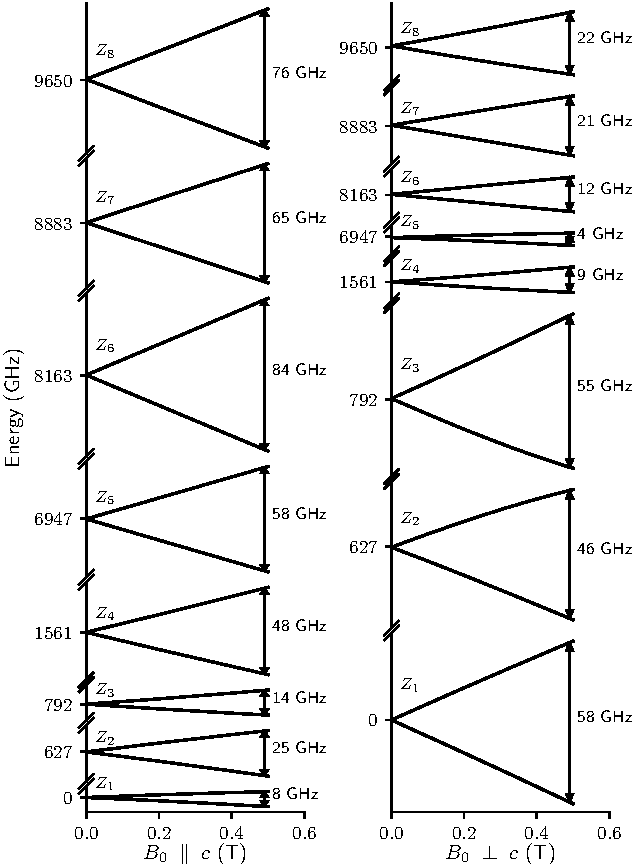
\includegraphics{chapter2/figures/energy_levels_vs_Bz_all.pdf}
    \caption{Energy levels for all $Z_i$ doublets under a magnetic field parallel (perpendicular) to the $c$-axis. The y-axis is broken to better show the magnetic splitting of the levels. Energy difference between the states of each doublet at 500~mT is shown as vertical double arrows, along with the approximate frequency of the transitiion}
    \labfig{energy_levels_vs_Bz_all}
\end{figure}

Under a magnetic field $\mathbf{B_0}$, the Hamiltonian of the ground $J=15/2$-multiplet can be written as 

\begin{equation}
    \label{eq:J-CF_Hamiltonian}
    \mathcal{H}_J = \mu_B \ g_J\mathbf{B_0}\cdot \mathbf{J} + \mathcal{H}_{\mathrm{CF}},
\end{equation}

The first term represents the Zeeman interaction, where $\mu_B/2\pi = 13.996$~GHz/T is the Bohr magneton and $g_J = 6/5$ is the Landé factor for the \Er ground state. \reffig{energy_levels_vs_Bz_all} illustrates the magnetic-field-induced splitting of the energy levels along the $c$-axis, obtained by direct diagonalization of the Hamiltonian in Eq.~\ref{eq:J-CF_Hamiltonian}. Each $Z_i$ doublet splits into two levels, with an effective, anisotropic gyromagnetic tensor that varies for each doublet. This anisotropy is evident from the differing transition frequencies observed when a 500~mT magnetic field is applied parallel versus perpendicular to the $c$-axis. 

\subsection{Spin-1/2 approximation}

The energy separation between the $Z_1$ and $Z_2$ doublets is approximately 650 GHz, which corresponds to a temperature of 50~K. Thus, at the working temperature of 10~mK, only the $Z_1$ doublet will be populated. This doublet can be effectively treated as a spin-1/2 with an anisotropic gyromagnetic tensor,

\begin{marginfigure}
    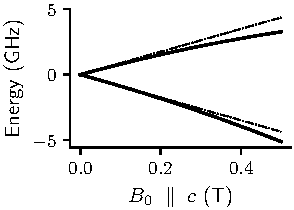
\includegraphics{chapter2/figures/energy_levels_vs_Bz_Z1.pdf}
    \caption{Energy levels of the $Z_1$ doublet as a function of magnetic field along the $c$-axis. The curves were obtaioned by direct diagonalization of Eq. \ref{eq:J-CF_Hamiltonian} and Eq. \ref{eq:er_spin_hamiltonian} (solid and dot-dashed resp.).}
    \labfig{energy_levels_vs_Bz_Z1}
\end{marginfigure}

\begin{equation}
    \label{eq:er_spin_hamiltonian}
    \mathcal{H}_S = \mathbf{B_0}\cdot \bar{\bar{\gamma}}_{^{3+}\text{Er}}\cdot\mathbf{S}
\end{equation}

with two eigenstates $\ket{\downarrow}$ and $\ket{\uparrow}$. The effective gyromagnetic tensor $\bar{\bar{\gamma}}_{^{3+}\text{Er}}$ is diagonal along the principal axes of the crystal, with values \sidecite{antipina.a._anisotropy_1981}

\begin{align}
\begin{split}
    \gamma_a = \gamma_b = \gamma_\perp &= -2\pi \times 117.3~\text{GHz/T}, \\
    \gamma_c = \gamma_\parallel &= -2\pi \times 17.45~\text{GHz/T}.
\end{split}
\end{align}

Throughout this thesis, we will primarily use this effective spin-1/2 approximation for the energy structure of the \Er. Nevertheless, it is important to note that as the magnetic field increases, mixing between doublets becomes significant, leading to deviations from the simple linear Zeeman splitting. This effect is illustrated in \reffig{energy_levels_vs_Bz_Z1}, where the energy levels of the $Z_1$ doublet are shown alongside the linear approximation as a function of magnetic field along the $c$-axis. Compared to the linear behaviour of the spin-1/2 approximation, the energy levels obtained from the crystal-field Hamiltonian "bend" as the magnetic field increases. A direct result of this non-linear behaviour is the appearance of a non-zero average magnetic moment

\begin{equation}
    \langle \mu_z \rangle = \frac{\partial E_\downarrow}{\partial B_0} - \frac{\partial E_\uparrow}{\partial B_0} \neq 0
\end{equation}

where $E_\downarrow$ and $E_\uparrow$ are the energies of the system as a function of the applied magnetic field $B_z$. This non-linearity is the origin of the pseudo-Zeeman \sidecite{baker_paramagnetic_1997} and pseudo-Quadrupole effects \sidecite{foley_secondorder_1947}, which are taken into account when interpreting the high-resolution spectroscopy experiments detailed in \red{labch}

\section{Spins coupled to a cavity}
\labsec{spins_coupled_to_a_cavity}

Spins coupled to a cavity text here.